\documentclass[]{IEEEtran}
\usepackage{url}
\usepackage{verbatim}
\usepackage{pgfgantt}
\usepackage{graphicx}
\graphicspath{ {images/} }
\usepackage{float}
\usepackage{multirow}
\usepackage{array}

% Title Page
\title{Planning and Design Document}
\author{Jay Ng, Suzanne Candanedo, Adam Dodson, Heather Clark, Amber Rosevear, Ash Brent-Carpenter}

\begin{document}
	\maketitle

	\section{Introduction}
	This document contains the plan, design and implementation details for the development of a virtual trading assistant for use by traders at Deutsche Bank. The software will take a query for information as input from the trader and output the requested information. The scope of the information returned is data related to the FTSE 100 and the news. The trading assistant will use artificial intelligence to become personalised for the user.
	
	\section{Methodology}
	Before commencing this project the options of software process models were carefully considered. The core functionality of the system (identified as must have requirements in the Requirements Analysis Document) will be developed using a waterfall style plan based methodology incorporating software reuse. For any features that are not considered core the agile model will be used.
	
	The plan based approach allows for increased planning and research time throughout the project, as well as time for the team to become comfortable with useful software engineering tools. The project requires multiple reports to be produced explicitly defining the specification, which matches the waterfall model of defining the entire project immediately. The tasks can be easily segmented so that every member of team can contribute. Due to the short timespan of the project, major drawbacks to the waterfall method such as changing technologies and business priorities are not a concern.
	
	Reuse of software will result in development will be streamlined, and eliminate time spent implementing pre-existing software. In addition, this also reduces the monetary cost of a project since resources are not allocated to unneeded projects.
	
	While having a waterfall based plan ensures that the project will be completed within the time limits, also using agile for functionalities not considered core results in maximum flexibility for adding extra features and improvements. Using a partly agile approach also mitigates a main flaw of the waterfall method and means that any potential additional requirements can be addressed, and the resulting changes can be documented and justified in the final report. Agile would not be suitable for the entirety of this project as there is not the time for multiple versions and limited opportunity for continuous customer feedback. 
	
	\section{Process Documentation}
	Development will take place over the course of 9 weeks from January 8th 2018 to March 9th 2018. During the initial stages of the project (until February 9th) the team carried out research into the specification and conversed with the customer to produce a Requirements Analysis document. Research was also conducted into the components that could be used to implement the system, and how these components would interact. The most appropriate discovered components were chosen for the design and implementation of the system, which is summarised in this document. 
	\begin{figure}[h]
	\begin{center}
	
	\begin{ganttchart}[vgrid, 
		bar/.style={fill=gray!50}, 
		bar height=0.2, 
		y unit chart=0.5cm, 
		y unit title=0.5cm, 
		x unit  = 0.4cm, 
		milestone label font=\footnotesize,
 	    group label font=\footnotesize,
        title label font=\footnotesize, 
        bar label font = \scriptsize]{1}{15}
		\gantttitle{February}{15} \\
		\gantttitlelist{8,...,22}{1} \\
		
		
		%First Group
		\ganttgroup{Front End Development}{1}{8} \\
		\ganttbar{Finance Data Collector}{1}{4} \\
		\ganttbar{Finance Analysis}{3}{6} \\
		\ganttbar{User Interface}{1}{7} \\
		\ganttbar{User Habit Analysis}{5}{8} \\
		\ganttbar{Alerts and Notifications}{5}{8} \\

		\ganttgroup{AI}{8}{15} \\
		\ganttbar{Qualitative Reasoning}{8}{12} \\
		\ganttbar{Automated Queries}{12}{15} \\
		
		\gantttitle{February}{5}
		\gantttitle{March}{10} \\
		\gantttitlelist{23,...,28}{1}
		\gantttitlelist{1,...,9}{1} \\
		
		\ganttgroup{Testing}{1}{8} \\
		\ganttbar{Testing}{1}{5} \\
		\ganttbar{Final Testing}{5}{8}\\
		
		\ganttbar{Documentation}{7}{13}\\
		
		%Third Group
		\ganttgroup{Final Stages}{10}{15} \\
		\ganttbar{Showcase practice}{11}{14} \\
		\ganttbar{Showtime}{14}{15} \\

		\ganttmilestone{Project Hand-In}{15}
		\end{ganttchart}

\end{center}
\caption{Gantt Chart representing the timeframe for each part of the project}
\end{figure}

The preceding plans are an overestimation of the amount of time it will take to complete each part of the project. This is to allow for a buffer in the case of setbacks. 
	
	\section{Risk Analysis}
	For this project, a risk is split into four risk ratings: low, medium, high and extreme which are represented by number ranges 1-2, 3-6, 7-10 and 11-12 respectively. These are calculated based the likelihood of the risk occurring (improbable, possible, probable) and the severity (acceptable, tolerable, undesirable, intolerable). \cite{risk}
	
	\begin{table*}[h]
	
	\begin{tabular}{| m{4cm} | m{1cm} | m{9.5cm} | m{1.5cm} | }
	
		\hline
		
		Risk & Inherent Risk Rating & Risk Management: avoidance, minimisation and contingency plans & Residual Risk Rating \\ 
		
		\hline
		
		Loss or change of team members [Project] & 
		6 & 
		Avoiding having unfinished work close to the deadline eliminates other team members being forced to complete extra tasks on short notice. Use of a plan based process model results in well-documented work, and any role can be taken over by another person if necessary. &
		1 \\
		
		\hline
		
		Change of management [Project and business] & 
		4 & 
		Keep the entire group updated with the current state of the project: remain in contact with the customer, attend lectures, and check the project page and forum. Plan for this by overestimating the time tasks will take. & 
		1 \\
		
		\hline
		
		A change in Requirements [Project and product] & 
		7 & 
		Have slack built into time estimates for every deliverable so there is time for further features to be created. & 
		3 \\
		
		\hline
		
		Losing focus on core requirements [Project] & 
		5 & 
		Focusing solely on the must have requirements until a functional system that will satisfy the customer is completed. Project manager needs to maintain contact with the rest of the group. & 
		2 \\
		
		\hline
		
		Planning fallacy (underestimation of the work required to complete the project) [Project and product] & 
		9 & 
		The project manager constantly engaging with team members that have not been participating should keep people focused on completing their tasks. Any optional components can be cut during the development cycle to focus the group's effort on the core functions.
		
		 Ensure plan has a short critical path and plenty of float time for optional components. & 
		2 \\
		
		\hline
		
		Data loss [Product] & 
		9 &
		Avoid relying on one person alone to be responsible for all of the project's data. Saving several copies of the entire project in different locations and using backups to cloud storage (e.g. github). & 
		1 \\
		
		\hline
		
		Required API unavailability [Product] & 
		10 & 
		Avoid making the software overspecialised for a specific API, so if another needs to be used in its place the software can quickly be adapted to the replacement API without major loss to functionality. 
		
	Modularise access to APIs so that data transfered to other modules are consistent. Consider alternatives that can be quickly subbed in. & 
		1 \\
		
		\hline 
		
		Technology changes, large updates to underlying systems [Business] & 
		6 & 
		Keep up to date on project-related technology changes by monitoring developer focused news. Have enough slack in the allocated time for the task so the system can be updated to be compatible with the new technology. & 
		4 \\
		
		\hline
		
		Hardware failure [Project] & 
		4 & 
		Having backup hardware, or an alternative solution. Avoid total dependence on a specific type of hardware by making the software compatible with several distinct types. &
		1 \\
		
		\hline
		
		Version control leading to incompatibility [Product] & 
		5 & 
		Repositories for previous version in the case of feature incompatibility to roll back to in the case of failure. The repository should have a master branch with the minimum viable product with separate branches adding features to avoid tainting the master branch. & 
		1 \\
		
		\hline
		
		Competition from other competing products [Business] & 
		7 & 
		Develop the project discreetly to avoid ideas and features being adopted by other teams. Utilise every team members skills effectively and efficiently to produce strongest possible solution. & 
		3 \\
		
		\hline
		
	\end{tabular}
	\caption{Table outlining project risks and management strategies}
\end{table*}
	
	\section{Design}
	
The chatbot will be a web based application. Thus, the system will be versatile compared to a traditional application as it will be compatible with any device with access to a modern browser. This is important as it will allow for fast development so the project will be completable within the required time period. Such a system will be straightforward to set up and run as computation is all performed remotely so there are minimal local requirements. It will also support expansion as updates and maintenance can be directly deployed to a server so the client will always be using the newest version. The chatbot requires an internet connection to function and being able to reliability connect to the host server is important. Thus it needs to be hosted by a service with a high uptime. This is why DigitalOcean’s servers will be used, as they have a history of reliably hosting systems with heavy traffic and computational power.

Taking an agile and modular approach to developing extra features results in an easily extendible program. Agile design allows flexibility in project requirements, and combined with extensive testing makes apparent any compatibility issues with the existing program. In addition agile developed projects are easily modulated and error tested. Errors for each section are caught because each section can be “targeted” and purposefully given invalid input. Testing and training the assistant to identify invalid input and to catch exceptions will make a system will large fault tolerance. 

Available APIs and libraries will be used to take advantage of existing code to allow for quicker development, prototyping, and testing or the application. Utilising a web platform also allows the creation of an intuitive user interface using any one of the many front-end libraries available on the web. APIs from Google and Python libraries will be used to take advantage of already existing scrappers and data collectors focused on the FTSE 100 stock and financial news.


	\section{System Architecture}
The software is a web-based Django app which gathers requested information via a hosted server. By design it is divided up into many distinct parts with interacting functions. A critical consideration for the design is that it does not collapse entirely when there is an error in one of these parts, and errors can be targeted without going through the entire program. To ease maintainability further the software is modelled using existing forms and not one developed solely for the project by the team. The overall system is best described using an event driven model, with the web application subsystem most easily adopted using a model-view-controller (MVC) pattern in the architecture of a Django app. 

\subsection{Overall Architectural Pattern}
The main function of the chatbot is to collect data for the trader; whether that be upon request or automatically. Both of these scenarios had to be considered when selecting a pattern, and an event-driven model architecture was found to be the best option.  Event driven model is the most appropriate for this software because since the software tracks a live feed of stocks, action occurs when there is a change in the state. For the requested information, event driven model matches the software’s information retrieval sequence: a new state is brought on by actions by the user or information being passed between subsystems.

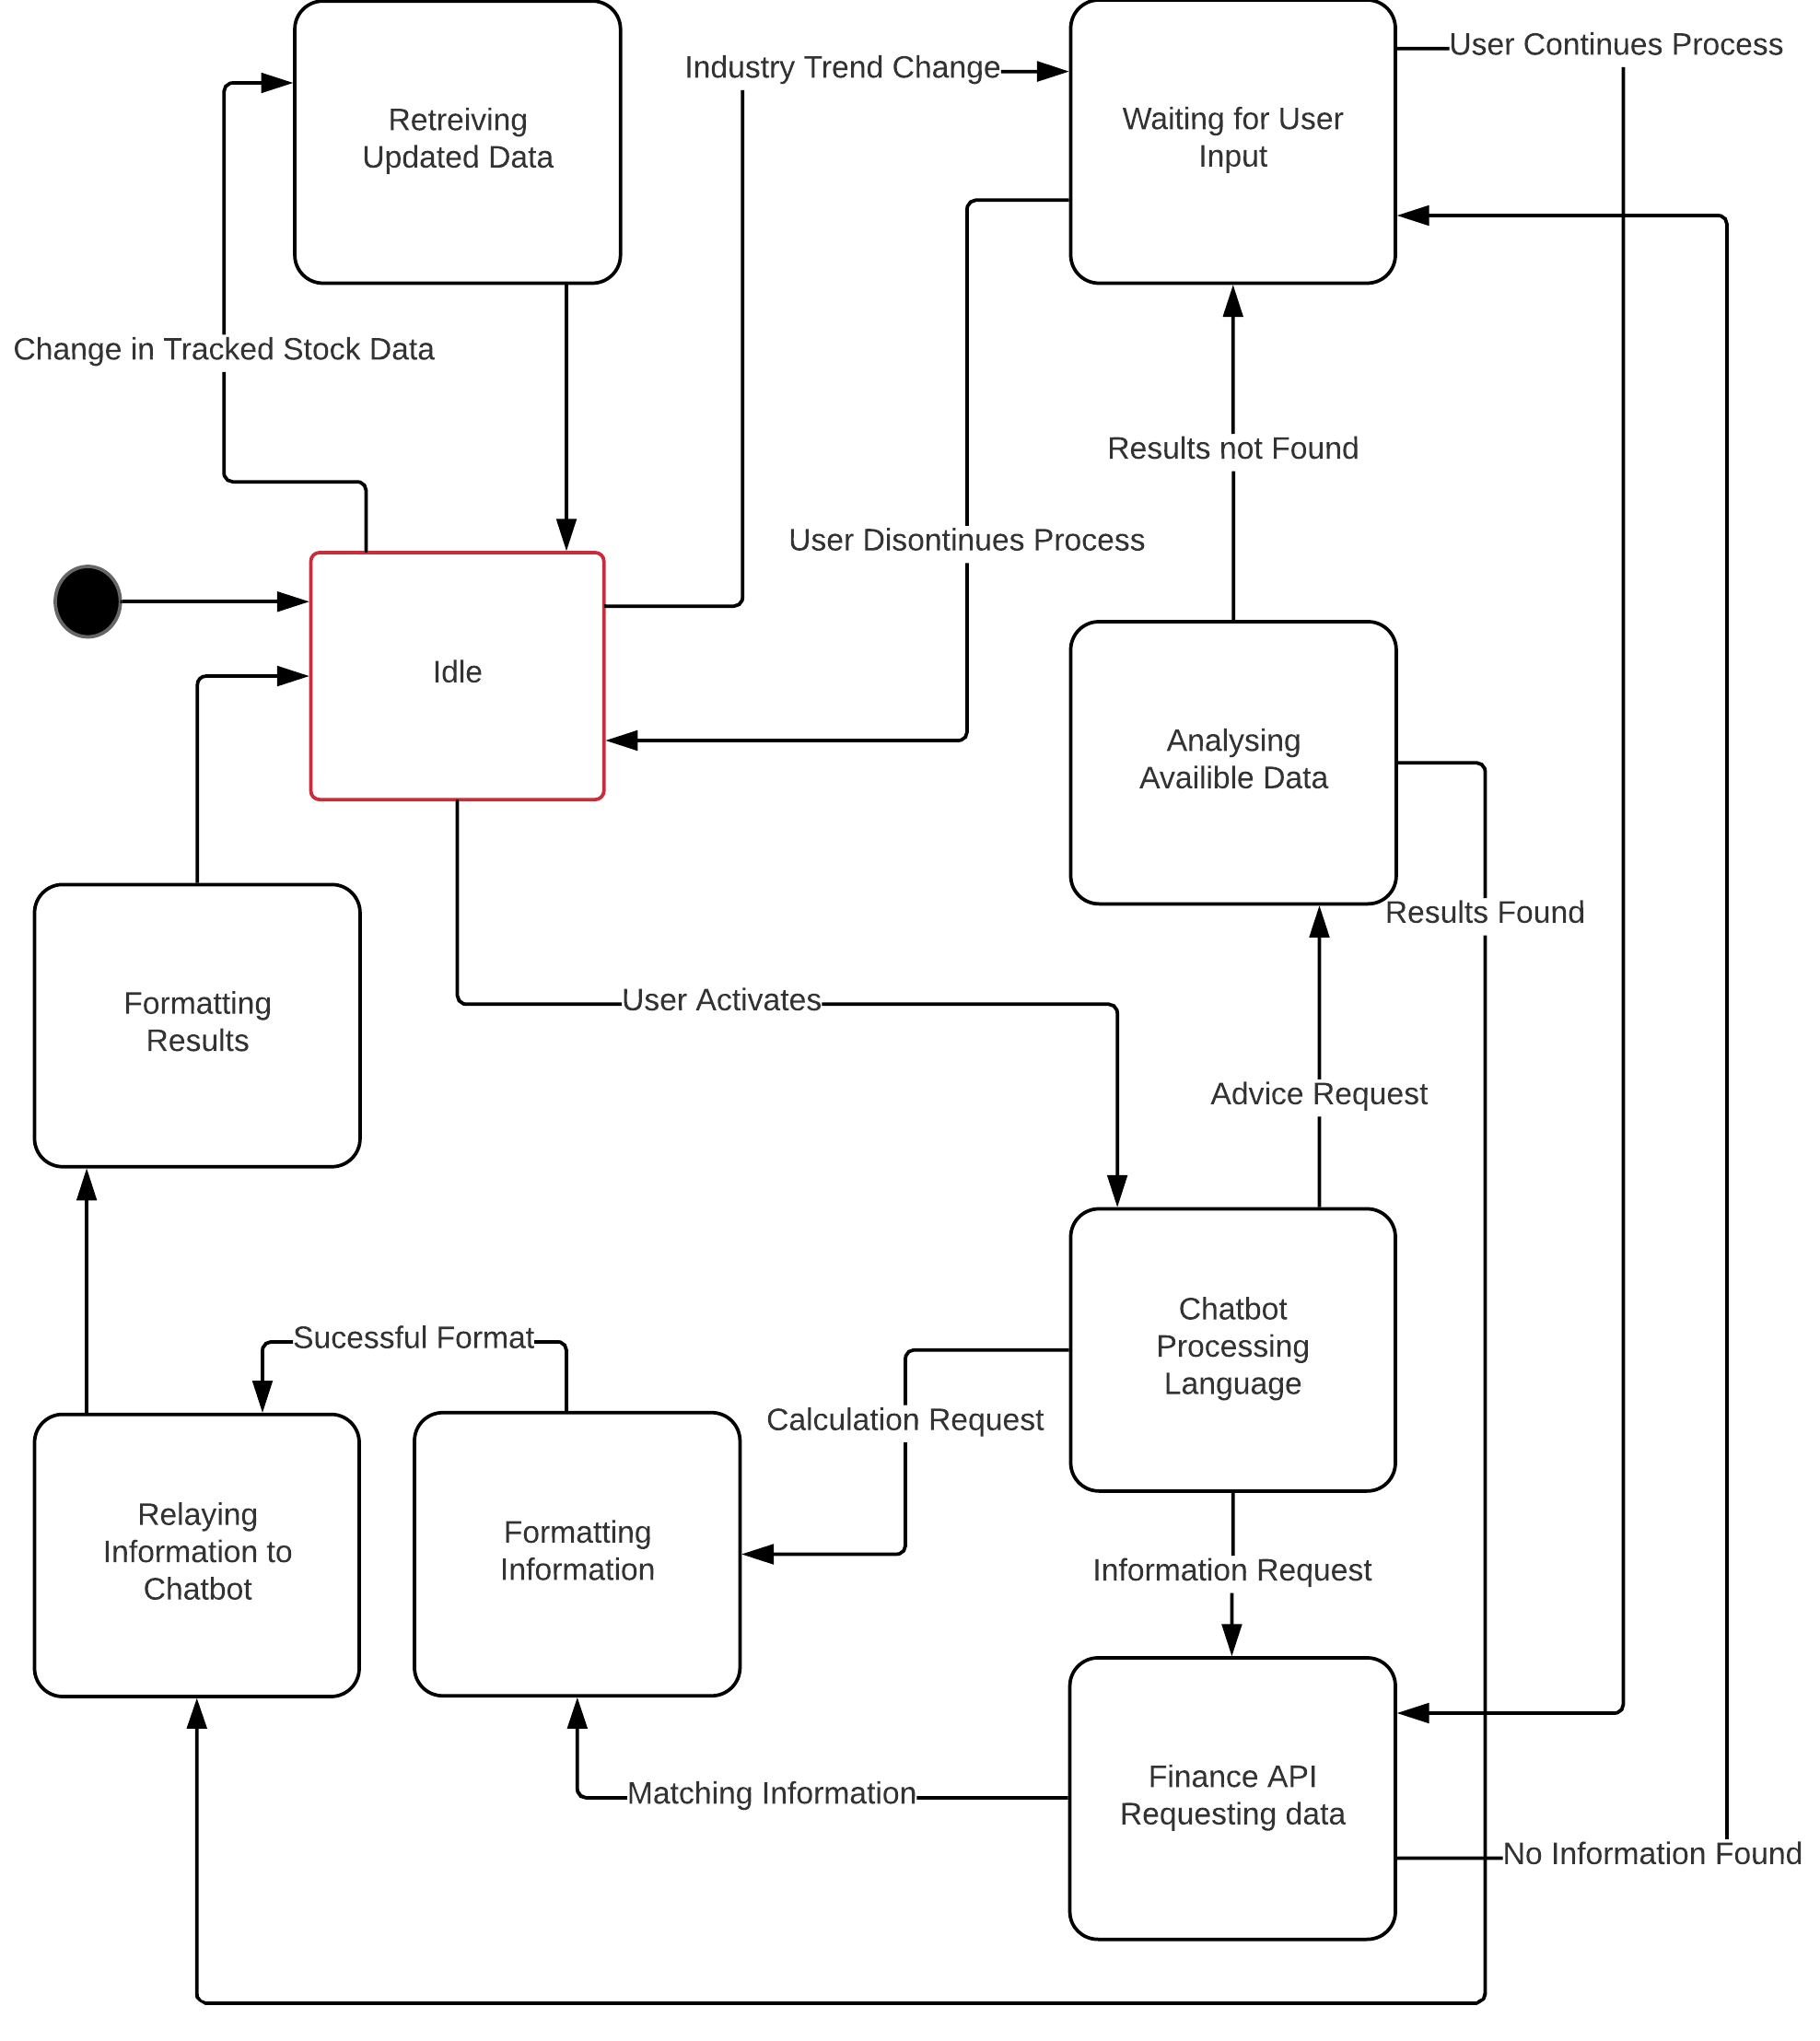
\includegraphics[scale=0.12]{BasicStateDiagram}

\subsection{Django Application Architecture Pattern}
Django adopts a Models, Template, Views (MTV) framework which follows the MVC architecture closely. A “template” in MTV is the presentation layer or what we call “views” in MVC. A “view” in MTV is the business logic layer or what we call “controllers” in MVC. It is therefore easy to adopt an MVC pattern in the architecture of a Django webapp. However, as UX/UI is not a main focus for the software, the bulk of data flow and processing is done server-side. Queries are handled using REpresentational State Transfer (REST) - a request is taken in GET/POST and a response is returned in AJAX/JSON. Therefore, the web app component is most appropriate as an MVC “micro” pattern.

The architecture of the charbot consists of three main parts. Firstly, our Models will be able to manage data, process queries, fetch APIs and other related calculations. Views consist of the UX/UI paired with the CSS framework that will be described in detail in later parts of this document. Finally, Controllers are in charge of handling asynchronous queries and answers and managing user interaction between the chatbot. The advantages of the MVC architecture in the context of chatbots include being able to modularise components for future iterations, time efficiency since each team member can focus on one part of the architecture independently and separation of concerns. Although the level of complexity in our design blueprint may increase using this architecture, one major reason why Django provides the perfect solution for a chatbot is the availability of advanced libraries in Python that complements the architecture.

\section{Implementation}
The Python programming language will be used to integrate the web server and business logic for the back end system. Using Python grants access to any of the Python ecosystem’s extensive libraries and tools \cite{python1} for ease of implementation. The web server will be created using the Django web framework \cite{django}, which is appropriate for a project of this scale and scope as it allows for fast prototyping and straightforward deployment.

As the chatbot will be web-based it must be hosted on a server. The chosen server that is reliable enough to satisfy the optimal system performance requirement and offers a variety of extra features is DigitalOcean \cite{digitalOcean}. DigitalOcean provides a cloud infrastructure suitable for demonstrating this prototype, providing the required level of performance using solid state drives and scalability using proper load balancing to manage a high number of requests. 

Stock data corresponding to FTSE 100 companies is stored in tickers, which must be retrieved by the program to gather requested information. FTSE 100 company tickers can be collected using python web scrapper libraries Beautiful Soup \cite{beauty} from any major financial websites providing tickers. Financial data and news regarding individual companies is collected via parsing tickers into existing APIs including Yahoo Finance and the London Stock Exchange using Pandas Data Reader \cite{panda}. Data collected should be cached and stored locally because the aggregate amount of data collected will be too large which will detriment software performance. The data collected must be asynchronous because the trader will require real time data to make informed decisions (i.e. < 0.5 seconds refresh time). Overall, speed and performance of collecting data is crucial as any small delays will be detrimental to a trader’s decision.

News concerning a specific company can be obtained using Yahoo Finance News Feed API in a reverse chronological order. From the news, a sentiment analysis can be performed on the attitude of the company. Sentiment Analysis is the quantitative analysis of public opinion and news surrounding the industry and company - used for identifying whether an industry value is going up/down. This can be done in three ways. Firstly, calculating the percentage change of a specific market index or a basket of ticker symbols from the same industry within a timeframe: i.e. the FTSE TechMark Index for the tech industry. Secondly, calculating the percentage change of a specific company within a timeframe. Lastly, using Natural Language Processing and machine learning python libraries Scikit Learn \cite{miks} on the news to identify key words and predict trends. 

Interpreting queries and language processing can be split into two main processes. Firstly, a master list of possible queries will be stored in a database. The prepared queries will start off simple with simple, non-compound queries (e.g. what is the price of company X) and will evolve into more advanced queries, hence the A.I. can be modularised and tweaked as desired by the trader in the future. Each query will be processed and analysed as described in later parts of this Planning and Design Document. Secondly, queries requested by traders will not match the exact phrase but should be semantically similar to the database of queries. Natural Language Processing Libraries \cite{spacy} \cite{tool} can rectify this issue by mapping a trader’s request to a suitable prepared query from the master list. Basic APIs from Google can deconstruct and select the keywords needed for mapping statements. Finally, autocorrect and regular expressions will be used to resolve human typing errors by traders.

\section{User Interface Design}

The user interface will use the Bulma CSS framework \cite{bulma}, to maintain a professional and consistent interface. The main non-design component of the user interface is a text query and response panel. Other components of the system will be added both in-line to the responses, and as separate frames of the interface. We chose to present the queries and responses in this manner as the style is akin to other chat based applications.

When designing the UI, many design principles will be considered, and each are outlined in \textbf{TABLE 2}.
	\begin{table}[h]
	\begin{tabular}{| m{2cm} | m{5.5cm} | }
		\hline
		Clarity & The information presented by the chatbot will be presented in a clear, readable and unambiguous way. The functionality of the different components of the site will be clearly labelled. The assistants response will be bolded to clearly differentiate user questions from the AI’s answers. \\
		
		\hline
		
		Compatibility & The system should be compatible with the operating system used by traders. It should also integrate nicely into the environment used at a trading desk, complementing other concurrent software such as the Bloomberg Terminal or Thomson Reuters Eikon. \\
		
		\hline
		
		Comprehensibility & Font sizes of approximate 12 and professional typography for easily legible text. \\
		
		\hline
		
		Consistency & Front-end design (layouts, fonts, colours) of the web application will be reused throughout the application. \\
		
		\hline
		
		Control & The user will be able to switch on/off notifications when necessary and decide when the assistant answers queries. \\
		
		\hline
		
		Efficiency & The assistant will respond with concise sentences limiting answers to 1 or 2 lines, together with clear diagrams to convey information as efficiently as possible. \\
		
		\hline
		
		Familiarity & The web application will make use of existing design and UI patterns to provide the user with a familiar interface. The query will be presented in a natural-feeling “chat” style. \\
		
		\hline 
		
		Recovery & Allow user to see query history with relevant timestamps. UI is simple enough to return back to the start state including the chatbot history and responses. \\
		
		\hline
		
		Responsiveness & When the AI is processing a request or when there is a problem connecting to the information sources, the UI will display a message reflecting the state of assistant. \\
		
		\hline 
		
		Simplicity & The color palette of the web application will be black, white and other muted colours, with the purpose of being as unobtrusive as possible in an already hectic environment. \\
		
		\hline
		
	
	\end{tabular}
		\caption{Table outlining the most important interface design considerations}
	
	\end{table}
	
	\section{System Models}
	
	System models are an easy way of representing how different aspects of a software interact with one another. Each model is a representation of an abstract aspect of the system, with a different perspective. The models are constructed to assist with clearly defining the functionality of the software for both the customer and the development team. For this project a Class Diagram\textit{Figure 2)}, a use case diagram \textit{(Figure 3)}, and a sequence diagram \textit{(Figure 4)}.
	
	\begin{figure*}[h]
		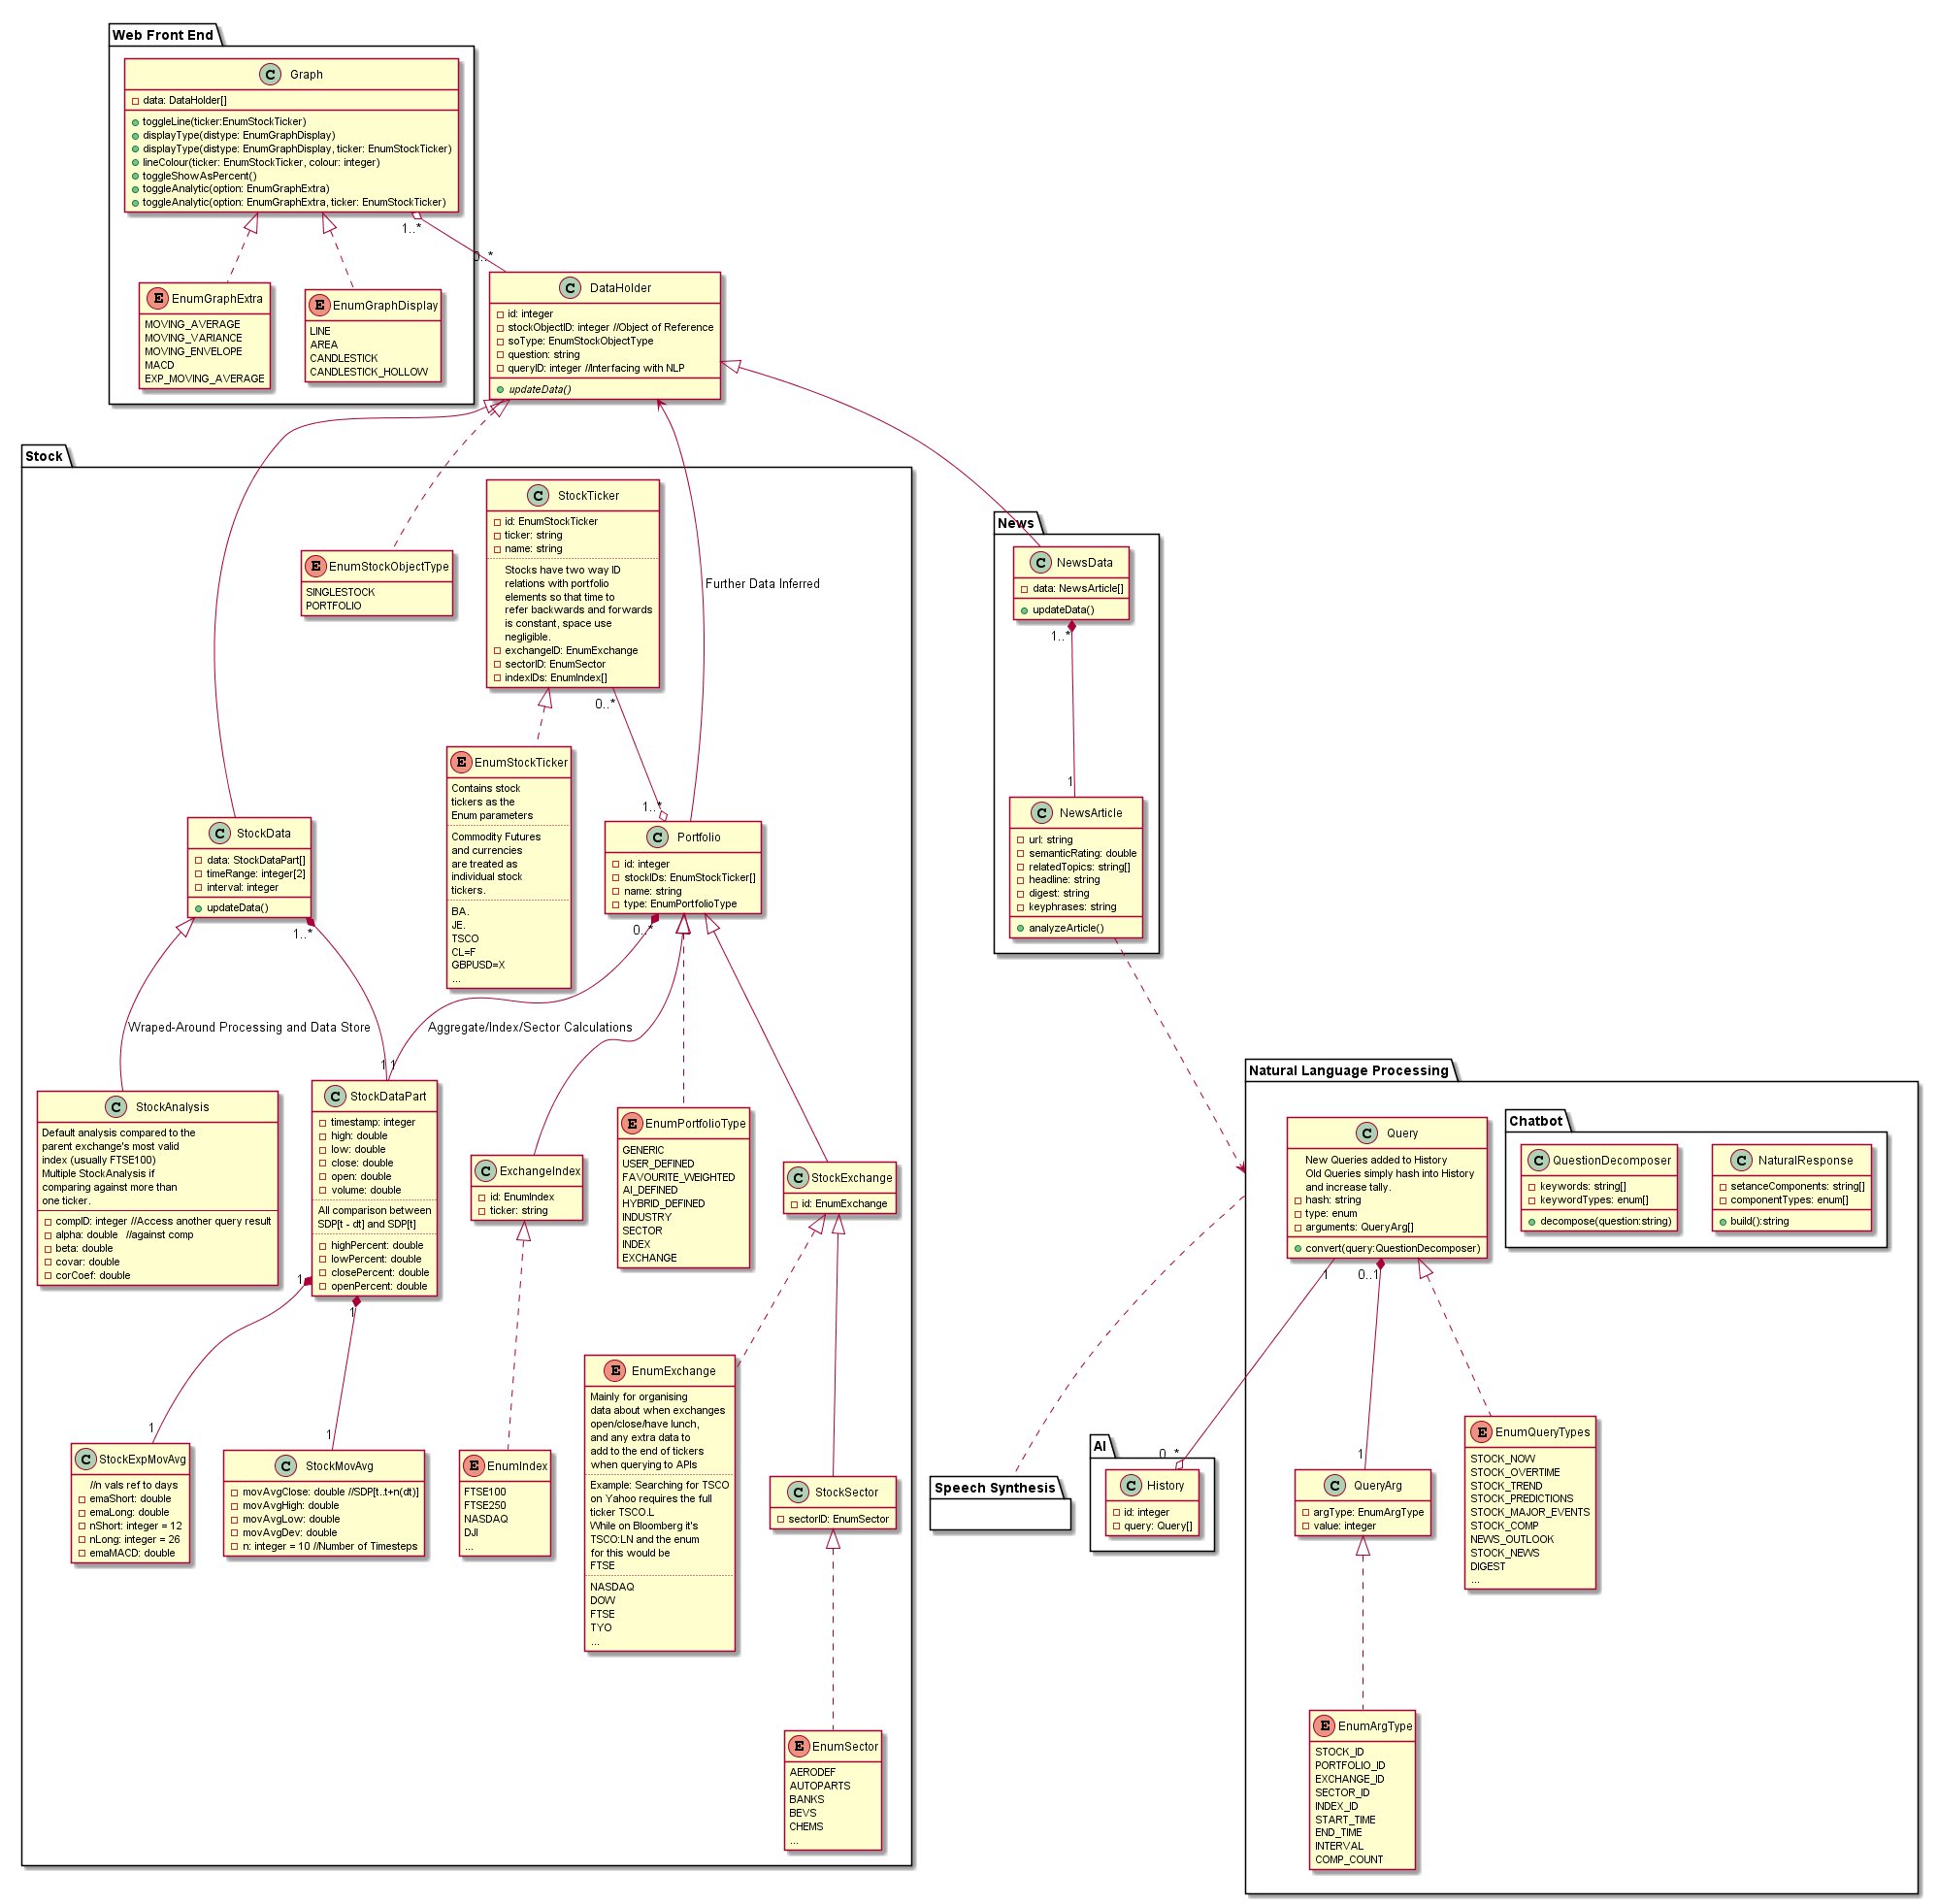
\includegraphics[width=\textwidth, height = 18cm]{classdiagram}
		\caption{The class diagram detailing the structure of the system via the classes}
	\end{figure*}
	
	\begin{figure*}[h]
		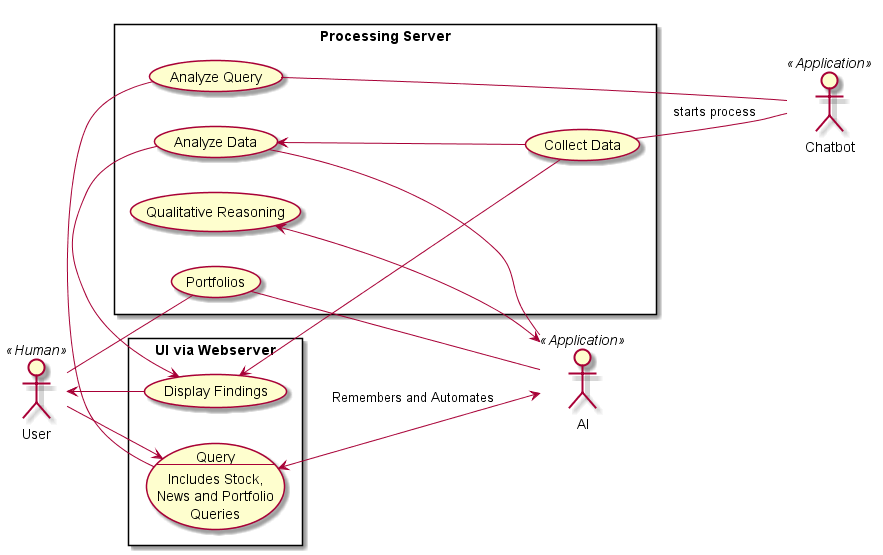
\includegraphics[width=\textwidth, height=10cm]{usecase}
		\caption{Use case diagram showing how the user interacts with the software}
	\end{figure*}
	
	These two models are focused on the coding and the user. The third system model is the sequence diagram, which is a detailed view of how each of the subsystems of the software interact with one another and when. The diagram traces the software from the moment a query is asked to the result being returned. This final diagram is located at the end of the document due to its size, labelled \textbf{figure 3 and 4}.
	
	\begin{figure*}[h]
		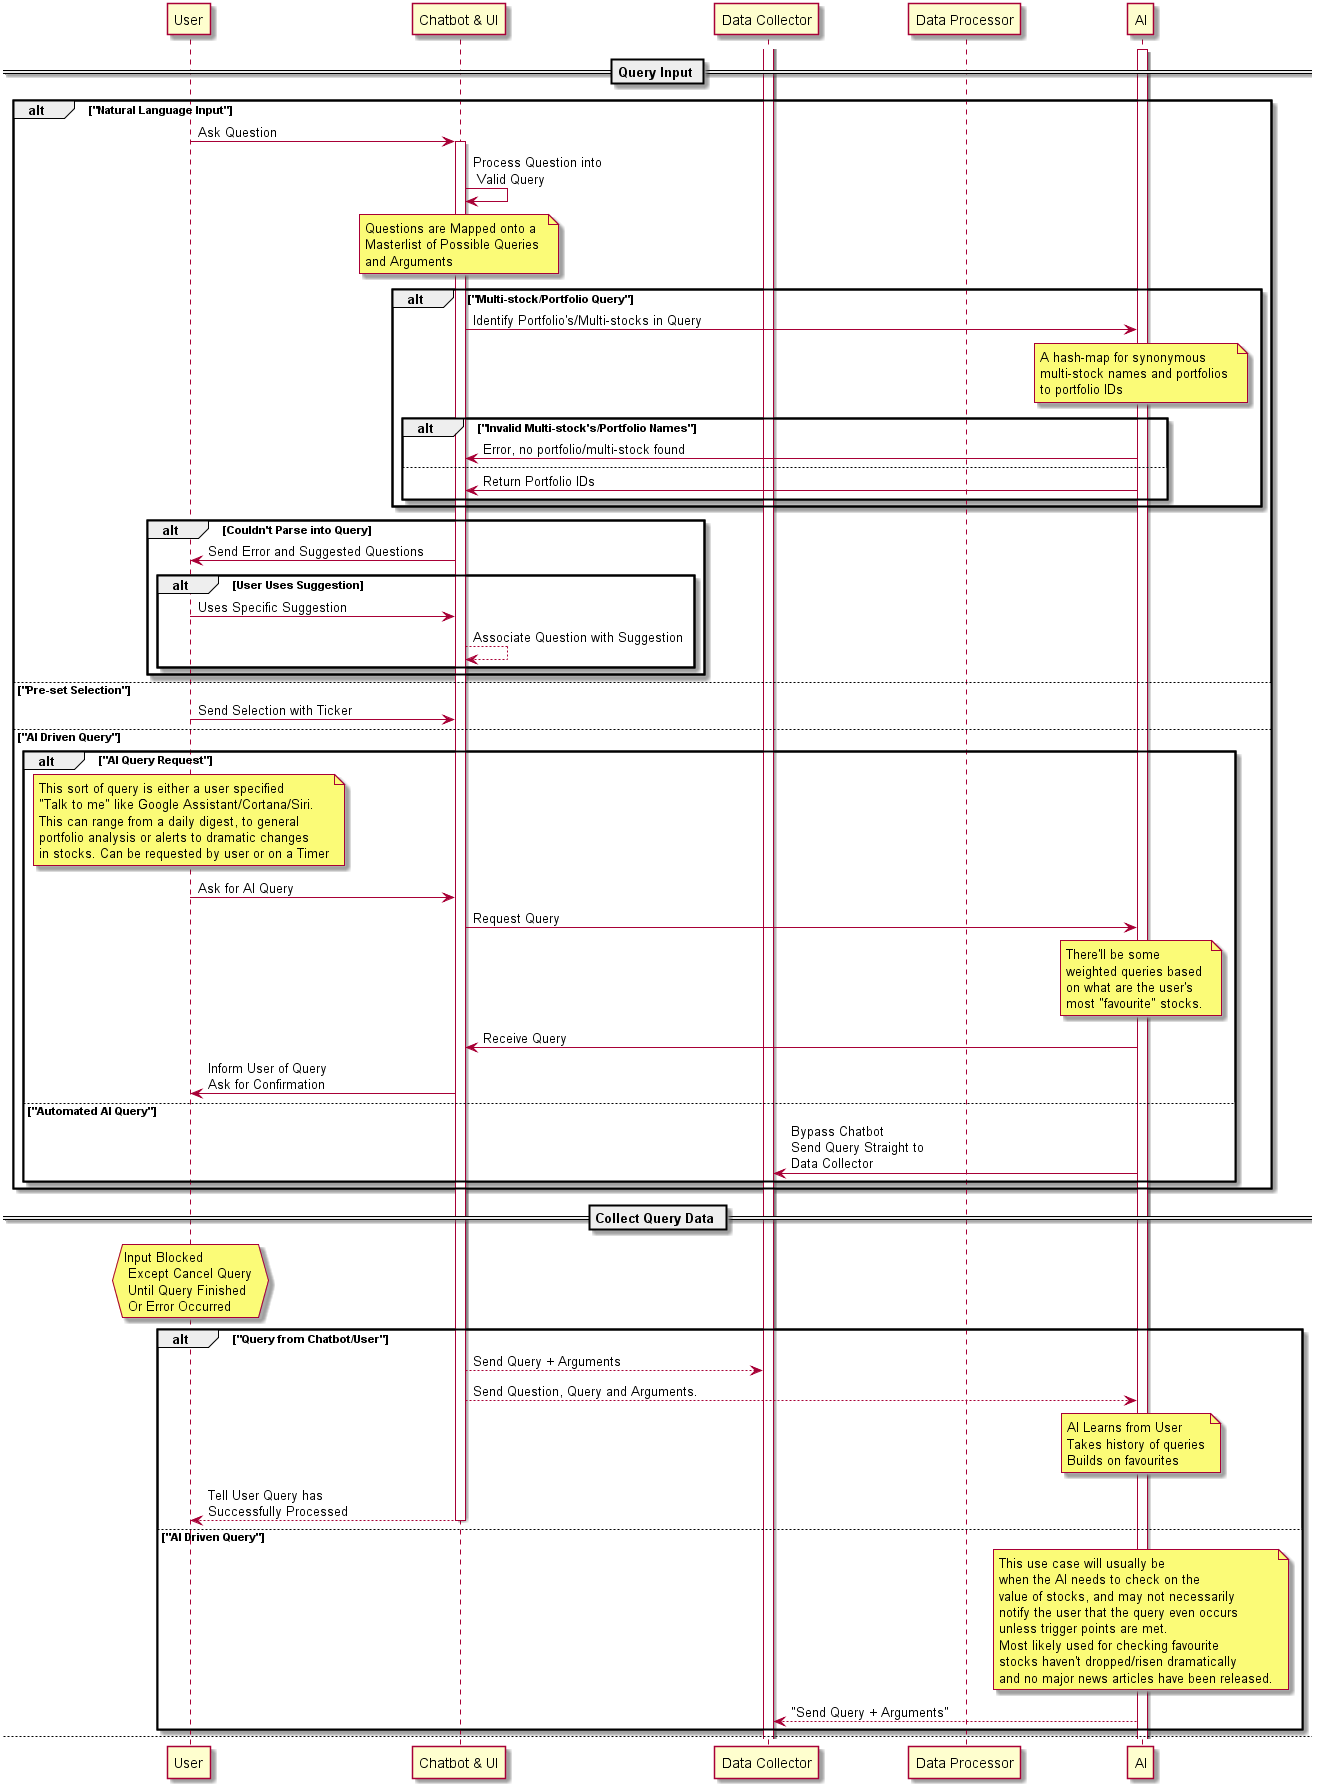
\includegraphics[width=\textwidth, height = 20cm]{sequence}
		\caption{Use case diagram the timing of system interactions and when they occur}
	\end{figure*}
	
	\begin{figure*}[h]
	
		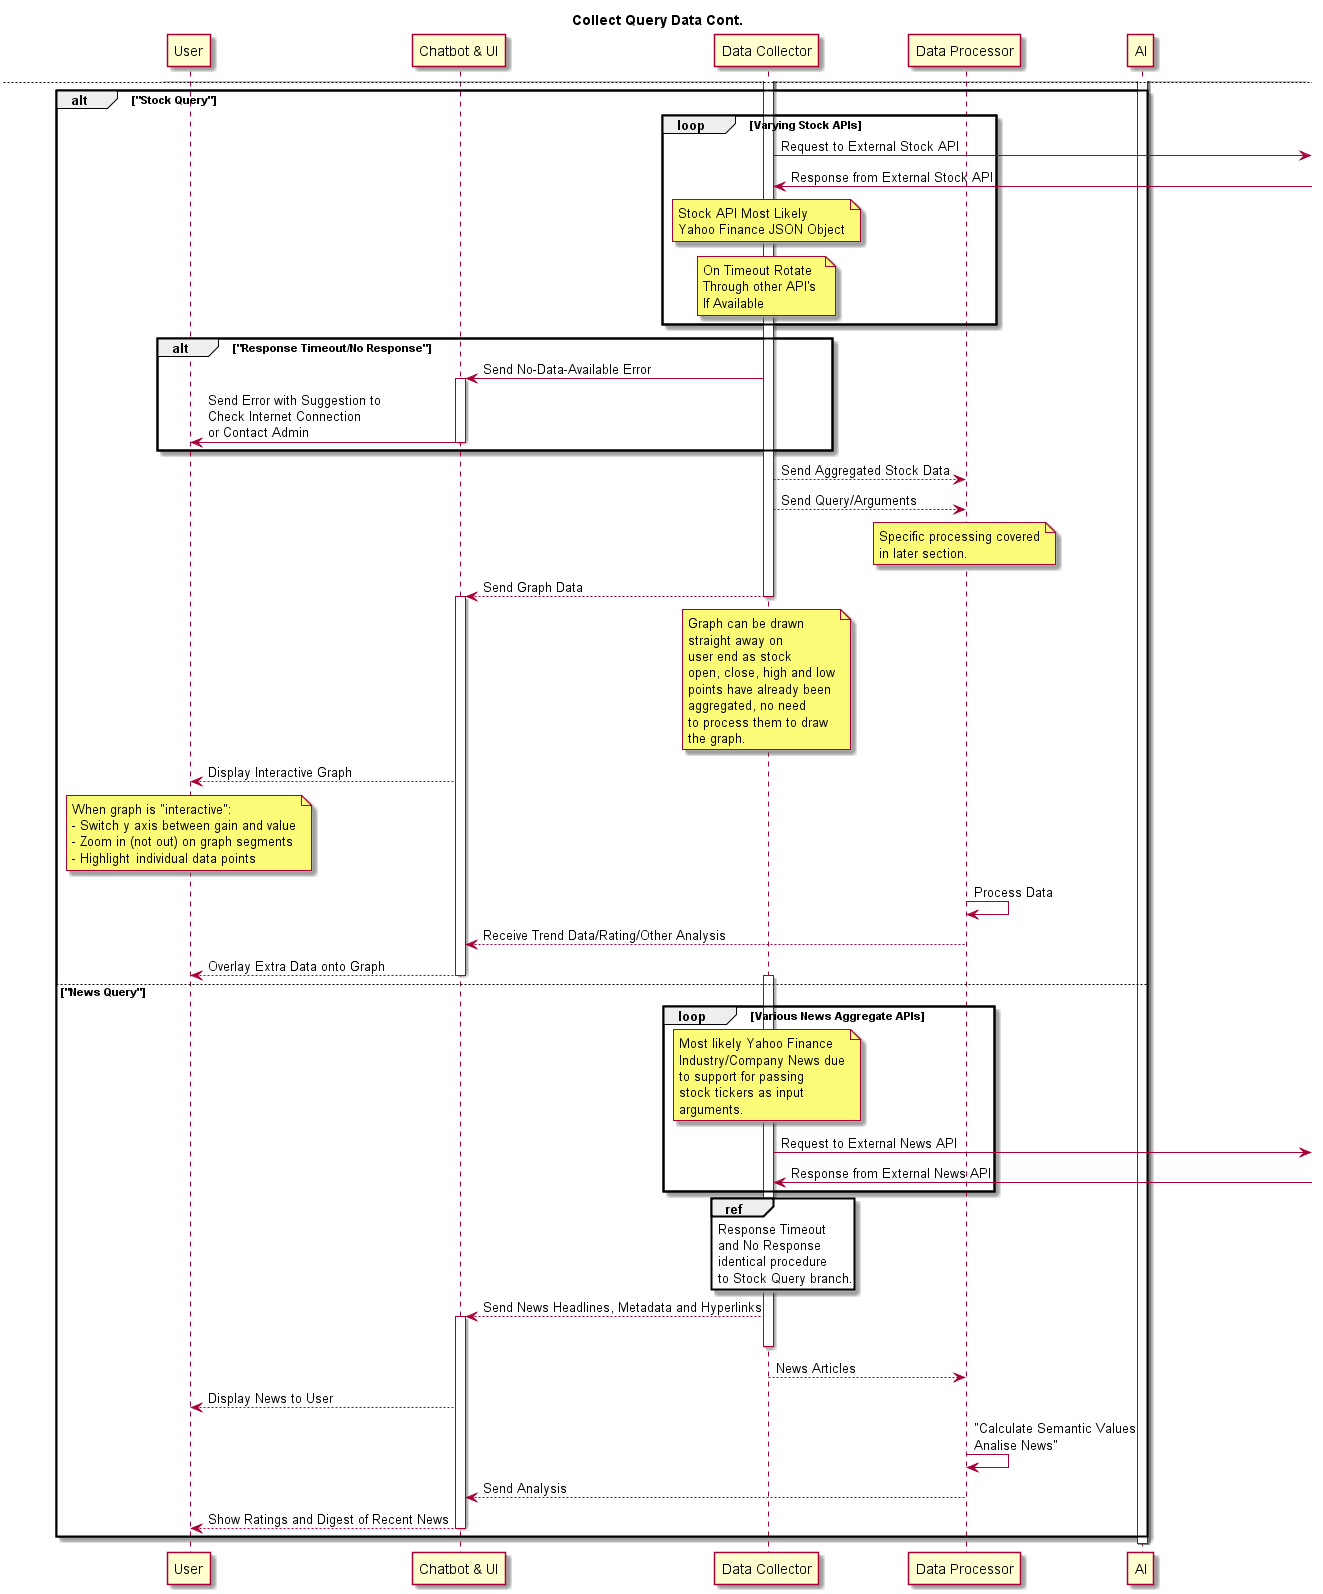
\includegraphics[width=\textwidth, height = 20cm]{sequence_001}
		\caption{Continuation of previous Case diagram}
	\end{figure*}
	
	
	
	
\mbox{} \\
\\\\\\\\\\\\\\\\\\\\\\\\\\\\\\\\\\\\\\\\\\\\\\\\\\\\\\\\\\
\\\\\\\\\\\\\\\\\\\\\\\\\\\\\\\\\\ \\\\\\\\\\
	
	\section{Testing}
	
	At the end of each phased process, the implemented design shall be tested. When an agile approach is used programming and testing will be performed concurrently.
	
	\subsection{Static Testing}
	The team will use Lightweight code review, due to time constraints and due to the prototype nature of the web application being created. Code review will be done in various points of the development process. Instances of pair programming during the development process will also allow mistakes in code to be caught earlier.  All source code produce will be peer reviewed by at least one other member of the team, who did not work on that code. Peer review will also be done with at least one of the original authors, who will explain the function and logic of the code, while another team member discusses possible errors and problems. The use of GitHub to store code will also allow all members of the team to be aware of changes made and allow them to review updates. Besides manual approaches, team members will also compile all code written to confirm its syntactical validity.
During code review, software verification shall be done through analysis. When a team member reviews code they will make logical evaluations to assure that the code is meeting the requirements set out in the requirement analysis report.
Development will also be externally validated by communicating with all stakeholders when issues arise.

	\subsection{Dynamic Testing}
	The results from inputs for the web application and input sections of the code will be tested against the expected outputs.
	
	\subsubsection{Unit Testing}
	As each member works on their segment of code, they will implement exploratory testing. The program will be run in order to verify that it is functional according to the requirements outlined in the requirement analysis report and adjust improvements as needed. The APIs used will be tested within the entire system, and in isolation. This will assure that the APIs not only function correctly on their own but are being used appropriately. Tests created at this point will be checked by injecting small faults in the program to assess if the testing methods are effective. Corner cases will be considered, and fuzzing test will be done; that is considering values that might be processed by the program but are not valid.
	
	\subsubsection{Integration Testing}
	At this stage each section of code has been proven to work individually. First, the AI and news and FTSE 100 information scraper should be able to interact properly. Once the issues between them are corrected, their interactions with the front end of the web applications can be tested. The purpose of these tests is to expose defects in the interfaces and their compatibility between them.
	
	\subsubsection{Integration Testing}
	Once the subsystems are able to exchange data without errors, it is now necessary to test if the correct information is being passed between them. Testing will be done by validating data before it is passed to another component. Data moved to another component will be logged to make sure that previous unusual or incorrect data does not affect the processing of a new input or the performance of the system.
	
	\subsubsection{System Testing}
	Once the whole system is integrated, it can be checked to see if it  the requirements set out in the requirements report. Specific test cases can be written down to check if the desired response is correct.
	
	\begin{table}[h]
	\begin{tabular}{| m{3cm} | m{5cm} | }
		\hline
		
		Test Case & Desired Response \\
		
		\hline
		
		“What is the current spot price for 3i Group?” & Spot price for 3i at the time request was sent \\
		
		\hline
		
		“What is the current trading volume for Carnival?” & Trading volume of Carnival at the time request was sent \\
		
		\hline
		
		“What is the percentage change in BP since the market opened?” & Percentage change of BP from current time the request was sent to the market opening price of the day request was sent. \\
		
		\hline
		
		“Has Astra Zenica risen this week?” & Yes or No, and negative or positive news about Astra Zenica \\
		
		\hline 
		
		“Are Pharmaceuticals rising or falling?” & Yes or No, and negative or positive news about the Pharmaceutical group \\
		
		\hline
		
		“How is Aerospace and Defense performing this morning?” & Poor or Well, and a percentage change of trading volume \\
		
		\hline
		
		“Which Utilities are rising right now?” & Industry member's names which are rising. \\
		
		\hline
		
		“What is the current spot price for Nestle?” & Informs user company is not in the FTSE 100 \\
		
		\hline
		
		“ “ & Informs user that input is not valid \\
		
		\hline
		
		“Haldfkja lafjl ladf” & Informs user that input is not valid \\
		
		\hline 
		
		“What’s the weather like today?” & Informs user that input is not valid \\
		
		\hline
		
		
	\end{tabular}
	\end{table}[h]
	
The usability of the system will be tested by presenting the web application to a group of users (who have some level of domain on financial terms and the FTSE 100) and presenting this users with a set of tasks to accomplish on the web application. While they attempt to perform the tasks, they be told to describe verbally their thought process and actions, while being monitored to see where it becomes difficult to understand the intentions of the software or the UI.
The systems will be checked to be compatible with various browsers; and especially the one preferred by Deutsche Bank traders.  

The system will be tested to measure how it handles various requests at a time by a trader, both valid and invalid requests. This process will also be checked to measure breaking points of the system and safe usage limits. Plus, it will help determine the stability of the system. Once having identified breaking points, the system will be checked to identify if it can recover from the crash or exception.

As specified in the Requirements Analysis, there are a couple of additional information that could be extracted such as the difference in currency and so on. Although these are not compulsory requirements, the attempt of implementing them will serve as a test to the scalability, reliability and performance of the basic software project.

When a change is made to the system once an error or bug has been detected, regression tests will be run. When a change is made the system is checked that it still has the same functions as before, and a new bug or error has not been introduced. This will be done through documentation which logs inputs to their results.

Sanity checks at each stage of the system testing will allow the team to quickly determine when and where tests are failing.

The success of the project will be measured not only through the tests described previously that detail if the original specification has been met, but also whether it meets the defined expectations. This is a qualitative measure that will be determined through conversing with the customer as much as possible throughout development and through the feedback given following the presentation delivery. 

\section{End of Life and Delivery}
	Software development will end after the ninth week, where the software will be presented to the client using a live demo. The critical and any implemented optional features will be displayed, and there will be a chance to ask the group questions about the developed software. The software will be in a fully functional state, ready for implementation by the client. 
	
\section{Conclusion}
	This software is explicitly designed to meet the design requirements. Throughout the document, many different aspects of the software's development were covered, starting from the risks taken and the earliest design to how the completed system will be tested. These points were elaborated and explained using a variety of UML diagrams presenting different views of the software. 

	
\bibliography{IEEEabrv,paddbib}
\bibliographystyle{IEEEtran}
\end{document}          

